\documentclass[10pt,a4paper,twocolumn]{article}
\usepackage[T1]{fontenc}
\usepackage[utf8]{inputenc}
\usepackage{lmodern,microtype}
\usepackage[margin=16mm,columnsep=6mm]{geometry}
\usepackage{amsmath,booktabs,tabularx,array}
\usepackage{graphicx,xcolor,tikz,pgfplots,balance}
\usepackage[font=small,labelfont=bf,skip=4pt]{caption}
\usepackage{titlesec}
\usepackage[hidelinks]{hyperref}
\pgfplotsset{compat=1.18}
\usepgfplotslibrary{groupplots,fillbetween}
\definecolor{blue}{HTML}{245581}
\definecolor{orange}{HTML}{BD5B21}
\definecolor{teal}{HTML}{187E78}
\titleformat{\section}{\normalsize\bfseries}{\thesection.}{.4em}{}
\titleformat{\subsection}{\small\bfseries}{\thesubsection}{.4em}{}
\titlespacing*{\section}{0pt}{8pt}{4pt}
\titlespacing*{\subsection}{0pt}{6pt}{3pt}
\setlength{\parindent}{1em}
\setlength{\parskip}{0pt}
\setlength{\textfloatsep}{8pt plus 2pt minus 2pt}
\setlength{\floatsep}{7pt plus 2pt minus 2pt}
\setlength{\intextsep}{7pt plus 2pt minus 2pt}
\renewcommand{\topfraction}{.95}
\renewcommand{\bottomfraction}{.85}
\renewcommand{\textfraction}{.05}
\renewcommand{\floatpagefraction}{.8}
\setcounter{topnumber}{4}
\setcounter{bottomnumber}{4}
\setcounter{totalnumber}{8}
\title{\vspace{-8mm}\Large\bfseries Brazil in a Global Atlas of Lyrical Themes:\\Verified Music Data and Social Context}
\author{}
\date{\vspace{-10mm}\small Data freeze: 11 October 2026}
\begin{document}
\raggedbottom
\maketitle
\begin{abstract}
\noindent We connect music to intimacy, gender, status, violence, digital access and cultural circulation. The archive contains 47.43 million source records; the verified geographical corpus contains 153,501 classified recording IDs in 68 markets. A fixed 55-market panel for 2017--2021 reveals broad growth of money, materialism, crime, weapons and territorial identity, alongside near-stable aggregate romance. Weapons increase in 53 markets. Brazil has the largest casual-sex increase and the second-largest explicitness increase in this panel. Romance declines in Top 200 but rises in Viral 50 for the same 52 markets. Fixed-sample social correlations retain distinct directions over five years. Seven figures, a full contextual matrix and an international atlas document these patterns and support reuse. The results identify changes in circulating repertoires, with Brazil as the focal case.
\end{abstract}

\section{Research question}
How do sexual, romantic, gender, material, and antisocial themes differ across music markets, and how do they relate to chart dynamics and external indicators? Brazil is a focal case, compared with other markets using the same measures. The analysis separates sexual content from objectification and misogyny, and thematic presence from endorsement. This allows several aspects of a song to coexist without collapsing them into one moral score.

The study combines historical charts, complete lyrics, structured Gemini classification, specialist verification, and dated contextual data. It addresses differences in the circulating repertoire, changes over time, and associations with economic conditions, gender inequality, homicide, internet access, and relative search interest. A market identifies where a recording charts; it does not identify the artist's nationality.

Six axes organize the analysis: \textbf{intimacy} (romance, heartbreak, reciprocity and sexual relations); \textbf{gender and power} (agency, objectification and misogyny); \textbf{status and inequality} (money, materialism and wealth); \textbf{violence and security} (crime, weapons and drugs); \textbf{digital environment} (access, search and connectivity); and \textbf{cultural circulation} (identity, genres and chart persistence). Brazil is the focal case. The atlas lets every market inspect its own profile, position and coverage.

\section{Corpus and method}
\subsection{Sources, units, and coverage}
Table~\ref{tab:sources} inventories the unified source catalog~\cite{archive}. MGD and Kaggle preserve overlapping Spotify charts; 19,942,141 exact native-ID equivalences were identified in the earlier overlap audit. Their row counts are therefore not additive evidence of independent events. We normalize Spotify recording IDs and count each ID once per market for the all-history comparison, and once per market--year for the annual comparison. Top 200 and Viral 50 are combined to describe the broader chart repertoire; source-specific results remain available separately.

\begin{table}[t]
\caption{Source archive before analytical deduplication. Counts include source territories; they are not audience sizes.}
\label{tab:sources}
\centering\footnotesize\setlength{\tabcolsep}{3pt}
\begin{tabularx}{\columnwidth}{@{}Xrr@{}}
\toprule Source / chart & Records & Period \\
\midrule
MGD / Spotify Top 200 & 21,257,472 & 2017--22 \\
Kaggle / Spotify Top 200 & 20,321,904 & 2017--21 \\
Kaggle / Spotify Viral 50 & 5,851,610 & 2017--21 \\
YouTube / popular videos & 3,037 & Sep. 2026 \\
Pro-M\'usica / aggregate & 50 & Aug. 2026 \\
\midrule Total stored source records & 47,434,073 & \\
\bottomrule
\end{tabularx}
\end{table}

The geographical analysis excludes GLOBAL, Hong Kong, and Puerto Rico under the established market policy, and keeps Taiwan as a separate market. The resulting union contains 222,102 distinct recording IDs, 652,121 recording--market pairs, and 386 market--year cells in 68 markets. Classified links cover 153,501 recording IDs and 461,447 recording--market pairs. The latter coverage is 70.8\%; individual market coverage ranges from 59.7\% to 79.1\%. Markets enter displayed comparisons with at least 300 classified recordings. Chart coverage and classification coverage are different quantities.

The main window starts on 1 January 2017 and ends on 13 March 2022. The partial 2022 repertoire is described but excluded from annual contextual correlations and search models. The 2026 YouTube and Pro-M\'usica captures are supplementary inventories, not extensions of the historical series. A YouTube video remains a video-level item, and the most-popular endpoint is not a historical YouTube Music Top Songs archive. Chartmetric pilot files and source capability records are retained as acquisition evidence, outside the quantified source union.

\subsection{Classification and completed verification}
Lyrics are acquired through the configured provider cascade, with source, version, and SHA-256 text hash preserved. Gemini receives the supplied lyric text and returns schema-constrained JSON. The model is \texttt{gemini-3.8-flash}; the taxonomy and prompt are \texttt{lyrics-classification-v1} and \texttt{lyrics-classification-prompt-v2}. The contract contains 26 ordinal dimensions in six groups: sexuality, relationships, gender representation, material status, antisocial content, and territorial identity. It also codes consent, target gender, representation roles, and stance. Generation uses Vertex AI; batch outputs are reconciled into an append-only PostgreSQL history.

\begin{figure}[t]
\centering
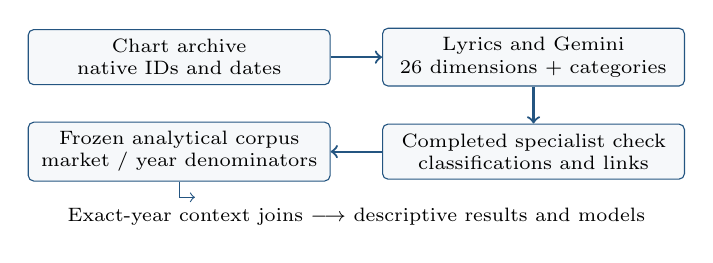
\begin{tikzpicture}[font=\scriptsize,box/.style={draw=blue,rounded corners=2pt,fill=blue!4,align=center,minimum height=7mm,text width=36mm}]
\node[box] (a) at (0,0) {Chart archive\\native IDs and dates};
\node[box] (b) at (4.5,0) {Lyrics and Gemini\\26 dimensions + categories};
\node[box] (c) at (4.5,-1.2) {Completed specialist check\\classifications and links};
\node[box] (d) at (0,-1.2) {Frozen analytical corpus\\market / year denominators};
\draw[->,thick,blue] (a)--(b);
\draw[->,thick,blue] (b)--(c);
\draw[->,thick,blue] (c)--(d);
\node[font=\scriptsize,align=center] at (2.25,-2.03) {Exact-year context joins $\longrightarrow$ descriptive results and models};
\draw[->,blue] (d.south)--(0,-1.78)--(.2,-1.78);
\end{tikzpicture}
\caption{Research workflow. Source records and model histories remain traceable; the analytical joins use explicit recording and time keys.}
\label{fig:workflow}
\end{figure}

Specialists completed verification of the classification results and the links between lyrics and recordings. This stage is complete. The analytical freeze uses the latest result per document for the fixed model, taxonomy, and prompt, then selects the latest applicable recording result. Text hashes, research authorization, and existing exclusion decisions define the eligible version. No confidence cutoff is applied to the reported corpus.

The freeze is 11 October 2026, 23:39 UTC (20:39 in S\~ao Paulo): 155,010 of 159,111 lyric documents are classified (97.4\%), representing 154,979 recording identities before selection. The selected corpus has 154,995 documents, 154,964 recording identities, and 154,942 linked native IDs before geographical restrictions. Errors, instrumental, ambiguous and other unscored states remain separate from score zero; full counts accompany the analysis.

Intensity is 0 (absent), 1 (incidental), 2 (substantial), or 3 (central). For dimension $d$, market $c$, and year $t$, substantial presence is
\begin{equation}
 P_{dct}=100\frac{\sum_{i\in A_{ct}}\mathbf{1}(s_{id}\geq2)}{|A_{ct}|},
\end{equation}
where $A_{ct}$ is the set of distinct classified recording IDs. Unclassified items are reported in coverage and omitted from the scored denominator. Scores describe the text, not the artist's conduct. Antisocial stance distinguishes condemnation, neutrality, ambivalence, normalization, and glorification; consent distinguishes mutual, ambiguous, coercive, nonconsensual, and non-applicable cases.

\subsection{Chart dynamics and external context}
Persistence counts native daily chart appearances, not uninterrupted streaks. Calendar span is reported separately. Daily Top-50 renewal is $1-J$, where $J$ is Jaccard similarity between two adjacent chart sets. We exclude non-adjacent dates from turnover summaries. Genre claims are derived from artist metadata and can overlap; their shares are not a mutually exclusive partition.

International trends use the same 55 markets in all five complete years, with at least 300 classified recording IDs and 50\% classification coverage in every market--year. Each market has equal weight; interquartile ranges describe market dispersion, not confidence intervals. The source sensitivities use 52 balanced Top-200 markets, 51 MGD-only markets, and 55 Viral-50 markets; the chart-family comparison uses the same 52 markets in both families. Additional panels require 70\% classification coverage throughout (8 markets), or pre-existing chart eligibility and a 1 January 2017 source start (46 markets). A distinct-recording yearly pool counts each ID once across the 55 markets. All denominators and membership lists are exported; partial 2022 is excluded.

Context is joined by exact market and reference year: World Bank income, Gini, unemployment, population and internet indicators; UNDP Gender Inequality Index (GII); OECD SIGI for its 2019 edition; and UNODC homicide indicators~\cite{wdi,gii,sigi,homicide}. Missing values stay missing, without interpolation. SIGI is not converted into an annual time series. OONI connectivity tests are kept separately from music and search measures. The contextual export verifies unique keys, value ranges, and raw-response hashes.

Google Trends exports retain term, language, query batch, sampling period, and raw hash. The historical panel has 2,150 series--year summaries from 383 local term/language/batch series. Means are weighted by the days represented by each bucket; weeks crossing years are split. Values reported as $<1$ contribute bounds $[0,1)$ rather than an invented point estimate. The index is relative search interest, normalized to the query's place and period, not visits or counts of people~\cite{trends}.

\section{Results}
\subsection{Thematic profile and market differences}
Figure~\ref{fig:themes} reports all 26 dimensions. Romantic affection (35.5\%) and heartbreak (21.4\%) are the most frequent substantial themes in the full selected corpus. Money references (16.5\%), reciprocity (14.1\%), drugs/alcohol (13.7\%), and materialism (13.5\%) follow. Sexual explicitness is 7.2\%, objectification 5.8\%, and misogyny 3.4\%. Themes overlap: their percentages do not sum to 100\%.

Brazil's all-history repertoire contains 7,186 classified IDs out of 9,619 charted IDs (74.7\% coverage). Romantic affection is 40.3\%, heartbreak 24.1\%, casual sex 15.1\%, explicitness 12.5\%, objectification 7.1\%, misogyny 1.9\%, and materialism 8.6\%. Brazil therefore combines comparatively frequent sexual and romantic content with lower misogyny and materialism than several comparator repertoires (Table~\ref{tab:markets}). Sexual content and misogyny do not move as one measure.

\begin{figure}[t]
\centering
\begin{tikzpicture}
\begin{axis}[width=\dimexpr\columnwidth-24mm\relax,height=107mm,scale only axis=false,
 xmin=0,xmax=50,ymin=.3,ymax=26.7,
 xlabel={Substantial thematic presence (\%)},
 xlabel style={font=\scriptsize},xtick={0,10,20,30,40,50},
 ytick={@@DIM_TICKS@@},yticklabels={@@DIM_LABELS@@},
 tick label style={font=\scriptsize},axis line style={gray},
 xmajorgrids=true,grid style={gray!18},tick align=outside,
 legend style={at={(.98,.98)},anchor=north east,font=\scriptsize,draw=none,fill=white},
 legend cell align=left]
\addplot[only marks,mark=*,mark size=1.9pt,color=blue] coordinates {@@ALL_COORDS@@};
\addlegendentry{Full corpus}
\addplot[only marks,mark=square*,mark size=1.8pt,color=orange] coordinates {@@BR_COORDS@@};
\addlegendentry{Brazil}
\end{axis}
\end{tikzpicture}
\caption{All taxonomy dimensions. The full corpus counts 154,964 selected recording identities once; Brazil counts 7,186 classified chart IDs once across the historical window. The full corpus is a pooled corpus reference, not an average national prevalence.}
\label{fig:themes}
\end{figure}

\begin{table}[t]
\caption{Selected circulation markets, pooled historical window. $n$: classified IDs; Cov.: classification coverage; E: explicitness; C: casual sex; M: misogyny; Mat.: materialism. All thematic columns are percentages at intensity $\geq2$.}
\label{tab:markets}
\centering\footnotesize\setlength{\tabcolsep}{3.5pt}
\begin{tabular}{@{}lrrrrrr@{}}
\toprule Market & $n$ & Cov. & E & C & M & Mat.\\
\midrule
@@COUNTRY_ROWS@@
\bottomrule
\end{tabular}
\end{table}

Across all 68 markets, the largest explicitness shares are in the Dominican Republic (21.4\%), Panama (19.2\%), and Chile (17.6\%). The largest misogyny share is in Romania (11.1\%); the largest materialism share is in Switzerland (27.8\%). These are distributions of charted recordings under a common coding rule, not rankings of national character.

Themes are distinct but overlap. Of 11,082 recordings with substantial explicitness, 60.1\% also have substantial objectification and 30.8\% misogyny. Among 20,943 materialism-positive recordings, 40.7\% also code crime; among 12,704 violence-positive recordings, 78.3\% also code crime. These conditional shares concern texts, not people. Consent, representation and stance remain separate measures in the accompanying distributions.

\subsection{Brazil over time and repertoire persistence}
From 2017 to 2021, Brazil's explicitness share rises from 7.0\% to 19.7\% and casual-sex share from 8.2\% to 23.8\%; romantic affection stays near 40--42\% (Figure~\ref{fig:brazil}). Classification coverage in those years ranges from 72.6\% to 76.1\%. These are changes in each year's repertoire; repeated recordings may enter several annual denominators. The 2022 partial window is shown separately and is not a full-year continuation.

\begin{figure}[t]
\centering
\begin{tikzpicture}
\begin{axis}[width=\columnwidth,height=53mm,xmin=2016.8,xmax=2022.2,ymin=0,ymax=50,
 xtick={2017,2018,2019,2020,2021,2022},xticklabels={17,18,19,20,21,22*},
 ylabel={Classified recordings (\%)},ylabel style={font=\scriptsize},
 tick label style={font=\scriptsize},ymajorgrids=true,grid style={gray!18},
 legend style={at={(.5,1.02)},anchor=south,legend columns=2,font=\scriptsize,draw=none},
 legend cell align=left]
@@ANNUAL_PLOTS@@
\draw[gray,dashed] (axis cs:2021.5,0)--(axis cs:2021.5,50);
\end{axis}
\end{tikzpicture}
\caption{Brazil's annual thematic shares. Classified denominators for 2017--2022: 2,228; 1,740; 1,234; 1,414; 1,412; 368. *2022 ends on 13 March. Lines connect annual summaries, not individual song trajectories.}
\label{fig:brazil}
\end{figure}

In the separate MGD Top-200 dynamics dataset, Brazil has 5,010 distinct recording--market pairs, with a median of 16 chart days (interquartile range 2--98), compared with 6 in the United States and United Kingdom, 7 in Germany, and 13 in Japan. Brazil's mean Top-50 Jaccard turnover is 0.069 across 1,892 adjacent daily chart pairs, against 0.114 in the United States and 0.032 in Japan. This supports a description of different repertoire persistence, without treating turnover as psychological anxiety.

Brazil's 2021 genre export contains 828 genre-annotated recordings: pop covers 25.6\%, agronejo 20.4\%, and arrocha 19.0\%. These overlapping artist-derived labels describe composition; they do not establish genre-adjusted thematic effects. Artist rankings and network files remain supplementary descriptions rather than additional independent song samples.

\subsection{International shifts and new patterns}
@@GLOBAL_TIME_FIGURE@@
@@GLOBAL_CHANGE_FIGURE@@
@@FAMILY_TREND_FIGURE@@

\textbf{Status and conflict gain repertoire share.} In the fixed 55-market panel, mean substantial money references increase by 4.50 percentage points (pp), drugs/alcohol by 3.80, materialism by 3.78, crime by 3.71, weapons by 3.53 and territorial identity by 3.12 from 2017 to 2021 (Figures~\ref{fig:global-time}--\ref{fig:global-changes}). Growth is geographically broad: weapons increase in 53/55 markets, crime in 51/55, territorial identity in 50/55, and materialism in 48/55. This is a shift in chart repertoire composition, not a claim that listeners changed their conduct.

\textbf{Romance persists while heartbreak grows.} Romantic affection averages 40.67\% in 2017 and 40.04\% in 2021; heartbreak rises from 22.18\% to 25.11\% in 44 markets. Sexual explicitness rises from 7.67\% to 11.25\%, whereas misogyny changes only from 2.71\% to 2.95\%. These trajectories separate affection, suffering, sexual content and gender hostility rather than treating them as one process.

\textbf{Mean growth can be geographically concentrated.} Sexual desire has a positive mean change (+2.31 pp), yet its median market change is $-0.09$ pp and only 26/55 markets increase. Large shifts in a subset of markets raise the mean. Figure~\ref{fig:global-changes} separates average magnitude from geographical breadth.

\textbf{Brazil's strongest shifts differ from the international pattern.} Brazil has the largest casual-sex increase in the 55-market panel (+15.63 pp), the second-largest explicitness increase (+12.73 pp, after Andorra), and the third-largest heartbreak increase (+9.68 pp, after Paraguay and Bolivia). Its weapons increase (+1.42 pp) is smaller than the international mean (+3.53 pp). Brazil's change therefore concentrates on sexual and relational themes rather than reproducing the strongest conflict trend.

\textbf{The aggregate masks chart-family divergence.} For the same 52 markets, romance falls by 3.29 pp in Top 200 but rises by 0.94 pp in Viral 50 (Figure~\ref{fig:family-trends}). Heartbreak grows in both (+4.24 and +3.06 pp), as do materialism (+2.78 and +1.11) and weapons (+3.52 and +2.56). Near-flat aggregate romance is therefore not evidence of an unchanged chart landscape. Misogyny also differs slightly in direction (+0.25 versus $-0.11$ pp).

Growth of materialism, crime, weapons, heartbreak and territorial identity persists in every source/coverage sensitivity. The distinct-recording pool also increases in these themes: materialism rises from 8.34\% to 15.88\%, crime from 7.03\% to 13.21\%, and weapons from 3.77\% to 7.71\%. Pool and market-mean levels answer different questions; shared recordings are not summed as independent global songs. Source-specific declines in romance remain explicit rather than being hidden by a single pooled statistic.

\subsection{Music and six social axes}
Within the 386 historical market--year cells, World Bank PPP income and internet use are observed in 380 cells each, GII in 372, Gini in 286, and total UNODC homicide in 332. SIGI is observed for 54 markets in 2019. These differences determine the pairwise sample sizes in Table~\ref{tab:context}.

All 26 lyric dimensions are crossed with 13 downloaded contextual indicators, separately in 2017--2021: 1,690 specified cells, of which 1,586 support descriptive correlations. The matrix includes observed and insufficient-data cells, without selecting only large coefficients. Table~\ref{tab:context} organizes selected contrasts across the six axes; the complete matrix accompanies the article.

\begin{table}[t]
\caption{Exact-year descriptive Spearman associations. $n$ counts markets; no causal or significance claim is assigned to these correlations. Income is per-capita PPP income; GII and SIGI are distinct gender indices.}
\label{tab:context}
\centering\scriptsize\setlength{\tabcolsep}{3pt}
\begin{tabularx}{\columnwidth}{@{}Xrrr@{}}
\toprule Lyrical theme / context & Year & $n$ & $\rho$ \\
\midrule
@@CONTEXT_ROWS@@
\bottomrule
\end{tabularx}
\end{table}

Materialism is positively associated with income ($\rho=0.408$) and negatively with Gini ($-0.456$) in 2021. Misogyny is negatively associated with GII in 2021 ($-0.330$) and SIGI in 2019 ($-0.459$), whereas objectification has weaker associations with both. Violence and crime shares are negatively associated with total homicide ($-0.261$ and $-0.253$). The direction and magnitude differ by theme and context; lyrical content is not a direct proxy for national violence or gender conditions.

\textbf{Intimacy} connects romantic affection and heartbreak to youth unemployment. \textbf{Gender and power} connects reciprocity and sexual agency to GII, with patterns distinct from misogyny. \textbf{Status} connects wealth symbolism to income. \textbf{Digital and cultural environments} connect explicitness to internet access and territorial identity to urbanization. Table~\ref{tab:context} reports every coefficient and sample size for these contrasts. OONI anomaly share has a near-zero association with explicitness. These are separate questions about representation, social conditions, infrastructure and circulation.

Brazil's 2021 contextual profile anchors the comparison: Gini 52.9, youth unemployment 28.3\%, GII 0.405, internet use 80.7\%, urban population 87.1\%, and total homicide 21.7 per 100,000. These actual downloaded values are joined to the same-year musical repertoire; they are not inferred from lyrics.

@@SOCIAL_TIME_FIGURE@@
\textbf{Social links persist across years, not just in a single cross-section.} Holding the market sample fixed within each pair, materialism correlates positively with PPP income in all five years ($\rho=0.41$--$0.61$, 54 markets) and negatively with Gini ($-0.50$--$-0.30$, 39 markets). Misogyny and GII remain negatively associated ($-0.55$--$-0.43$, 53 markets); violence and homicide also remain negative ($-0.43$--$-0.27$, 47 markets). Territorial identity and urbanization remain positive ($0.23$--$0.36$, 54 markets). Romance's link to youth unemployment is weaker ($-0.17$--$-0.04$, 53 markets). Figure~\ref{fig:social-time} shows these fixed-sample trajectories. The results challenge a direct reading of lyrical violence or misogyny as national social prevalence; they instead define concrete questions about repertoire selection, circulation and representation.

\subsection{Historical search associations}
The established search specification uses the English term \textit{porn}, selecting the lexicographically first query batch within each market before fitting outcomes. Local indices are standardized within each eligible market series. Models use 2017--2021, at least 300 classified recordings per market--year, at least 80\% temporal search coverage, at least four eligible years per market, and at least 20 markets. Native-language terms remain in the descriptive panel.

For each of ten focal dimensions, we estimate
\begin{equation}
 P_{dct}=\alpha_{dc}+\lambda_{dt}+\beta_d z_{ct}+\gamma_d^{\mathsf T}X_{ct}+\epsilon_{dct},
\end{equation}
where $z_{ct}$ is the standardized local search index, $\alpha$ and $\lambda$ are market and year effects, and adjusted models control log PPP income and internet use. Errors are clustered by market, with $t$ intervals. Baseline requires 50\% classification coverage (60 markets, 295 market--years); the 70\% sensitivity uses 24 markets and 104 cells; adjusted models use 59 markets and 290 cells. Benjamini--Hochberg correction covers all 30 estimated models.

\begin{table}[t]
\caption{Adjusted within-market search associations. Effect units: percentage points per local search-index standard deviation. All models have 59 markets and 290 market--years; intervals are 95\%; $q$ covers the 30-model family. Full baseline and 70\% sensitivity estimates accompany the manuscript.}
\label{tab:models}
\centering\scriptsize\setlength{\tabcolsep}{3pt}
\begin{tabularx}{\columnwidth}{@{}Xrrr@{}}
\toprule Outcome & $\beta$ & 95\% interval & $q$ \\
\midrule
@@MODEL_ROWS@@
\bottomrule
\end{tabularx}
\end{table}

No model meets $q<0.05$. Adjusted materialism is $-0.653$ points per local standard deviation (95\% interval $[-1.105,-0.201]$, $q=0.078$), and drugs/alcohol is $-0.578$ ($[-1.019,-0.138]$, $q=0.083$). Explicitness is $-0.491$ ($[-1.016,0.035]$, $q=0.285$). The 70\% sensitivity has wider intervals and does not retain evidence below the same threshold. The findings do not support a simple positive relationship between relative adult-term searches and sexual lyrical content. They also do not prove that no relationship exists.

\balance
\section{Interpretation and scope}
Music provides a measurable record of how intimacy, power, status, violence and identity circulate. Broad growth of status, conflict and territorial references coexists with persistent romance and rising heartbreak. Brazil's leading sexual and relational shifts differ from the international weapons trend. Chart-family divergence shows why one aggregate can conceal opposing processes. Repeated social correlations further show that musical representation does not map directly onto national social indicators. The search results add another dimension rather than defining the study.

The atlas makes these findings actionable for research and public debate: educators can compare representations, researchers can test mechanisms, and cultural institutions can track repertoire change with explicit evidence. It replaces broad judgments with inspectable measures. Each international position is specific to one dimension; no composite moral ranking is imposed.

Inference is bounded by the observed units. Charted songs are a selected repertoire, not a sample of residents; streams are not unique listeners or endorsement. Spotify chart streams use eligibility filtering~\cite{spotify}. Equal recording weights describe repertoire diversity, not listening exposure. Top 200 and Viral 50 have different selection mechanisms. Shared songs create dependence between markets that market-clustered errors do not fully remove. Short panels, changing repertoires, genre mix, and missing contextual values constrain interpretation even with completed specialist verification.

Adult-term search interest is not pornography consumption. OONI coverage comprises 211 market--year cells with connectivity-test counts; the tests come from participating networks and anomalies do not by themselves confirm censorship~\cite{ooni}. Female homicide is not synonymous with femicide, and partner/family homicide is a distinct indicator. The 2019 SIGI edition and annual GII must retain their own dates and definitions. Annual 2022 context extends beyond the musical cutoff and stays outside models.

Historical commercial visits, weighted WVS sexual-value aggregates and dated TikTok exposure are absent. Contemporary DNS and the traffic pilot remain separate. A legacy index combining historical song shares with 2024 population is synthetic, not an exposed audience estimate. Viral-50 membership does not identify TikTok effects on longevity.

\section{Reproducibility and conclusion}
The frozen analysis exports all 26 dimensions, thematic co-occurrence, country/year denominators, eight international panels, distinct-recording pools, fixed-sample social correlations, source-specific results, the complete 1,690-cell social matrix, and all 30 search models with samples and exclusions. The manifest records the database snapshot, model/taxonomy/prompt, hashes and completed specialist verification. Figures use this freeze; publication figures are also supplied as PDF, SVG and PNG.

The supplied scripts reproduce the frozen statistics, contextual matrix and standalone LaTeX figures without new model calls or database writes. The contribution is a verified comparison of music and society across several dimensions, supported by inspectable recording, market and year evidence.

\begingroup\scriptsize
\begin{thebibliography}{8}
\setlength{\itemsep}{1pt}\setlength{\parskip}{0pt}
\bibitem{archive} Chart Observatory. Local source inventory, MGD/Kaggle overlap audit, classification database, and frozen article manifest. Snapshot: 11 October 2026. Repository: PromiscuidadeMusical.
\bibitem{spotify} Spotify. \href{https://support.spotify.com/us/artists/article/understanding-spotify-charts/}{Understanding Spotify charts}. Accessed 11 October 2026.
\bibitem{trends} Google. \href{https://support.google.com/trends/answer/4365533?hl=en}{FAQ about Google Trends data}. Accessed 11 October 2026.
\bibitem{wdi} World Bank. \href{https://data.worldbank.org/}{World Development Indicators}. API responses for 2017--2022, retrieved 11 October 2026; endpoints and hashes in the context manifest.
\bibitem{gii} UNDP. \href{https://hdr.undp.org/data-center/documentation-and-downloads}{Human Development Report 2025: composite indices time series}. Historical GII observations, archived with provenance.
\bibitem{sigi} OECD. \href{https://www.oecd.org/en/topics/sub-issues/social-institutions-and-gender-index.html}{Social Institutions and Gender Index, 2019 edition}. Archived SDMX observations.
\bibitem{homicide} UNODC. \href{https://dataunodc.un.org/dp-intentional-homicide-victims}{UN-CTS intentional homicide data}. July 2026 release; historical years joined without imputation.
\bibitem{ooni} OONI. \href{https://ooni.org/support/interpreting-ooni-data/}{Interpreting OONI data}. Historical Web Connectivity aggregates and response provenance retained in the context archive.
\end{thebibliography}
\endgroup
\clearpage
\onecolumn
\section*{International atlas: all 68 circulation markets}
\noindent\small Position ranks sexual explicitness (E) from highest to lowest. Other columns retain their own values; the companion interactive atlas ranks any of the 26 dimensions. $n$ is the classified recording count; Cov. is classification coverage; R is romantic affection; C is casual sex; O is objectification; M is misogyny; Mat. is materialism; V is violence; Cr. is crime. All thematic values are percentages at intensity $\geq2$, pooled over 2017--2021 and through 13 March 2022. Each recording counts once per market. Higher position is a larger thematic share, not better performance. Brazil is the reference case.\par\vspace{4pt}
\centering
\fontsize{8}{9}\selectfont\setlength{\tabcolsep}{4pt}
\begin{tabular}{@{}rlrrrrrrrrrr@{}}
\toprule Pos. & Circulation market & $n$ & Cov. & R & E & C & O & M & Mat. & V & Cr. \\
\midrule
@@ATLAS_ROWS@@
\bottomrule
\end{tabular}
\end{document}
